% Generated by python3 -m squares.paper.figures; do not edit.
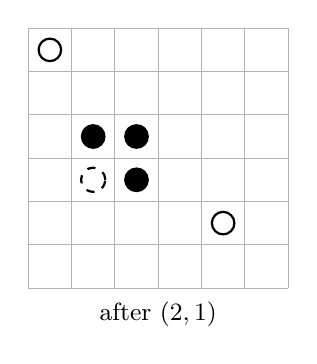
\begin{tikzpicture}[scale=0.55]
  \draw[gray!60] (0,0) grid (6,-6);
  \foreach \r/\c in {2/2, 3/2, 2/1}
    \filldraw[fill=black,thick] (\c+0.5,-\r-0.5) circle (0.26);
  \foreach \r/\c in {0/0, 4/4}
    \filldraw[fill=white,thick] (\c+0.5,-\r-0.5) circle (0.26);
  \draw[thick,dashed] (1.5,-3.5) circle (0.28);
  \node at (3,-6.6) {\small after $(2,1)$};
\end{tikzpicture}
\hspace{1em}
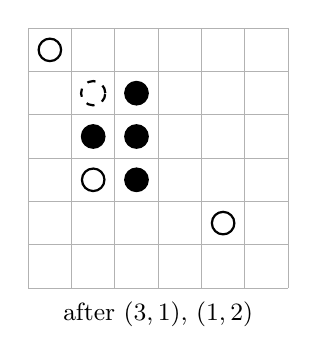
\begin{tikzpicture}[scale=0.55]
  \draw[gray!60] (0,0) grid (6,-6);
  \foreach \r/\c in {2/2, 3/2, 2/1, 1/2}
    \filldraw[fill=black,thick] (\c+0.5,-\r-0.5) circle (0.26);
  \foreach \r/\c in {0/0, 4/4, 3/1}
    \filldraw[fill=white,thick] (\c+0.5,-\r-0.5) circle (0.26);
  \draw[thick,dashed] (1.5,-1.5) circle (0.28);
  \node at (3,-6.6) {\small after $(3,1)$, $(1,2)$};
\end{tikzpicture}
\hspace{1em}
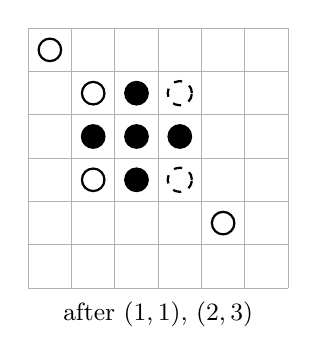
\begin{tikzpicture}[scale=0.55]
  \draw[gray!60] (0,0) grid (6,-6);
  \foreach \r/\c in {2/2, 3/2, 2/1, 1/2, 2/3}
    \filldraw[fill=black,thick] (\c+0.5,-\r-0.5) circle (0.26);
  \foreach \r/\c in {0/0, 4/4, 3/1, 1/1}
    \filldraw[fill=white,thick] (\c+0.5,-\r-0.5) circle (0.26);
  \draw[thick,dashed] (3.5,-1.5) circle (0.28);
  \draw[thick,dashed] (3.5,-3.5) circle (0.28);
  \node at (3,-6.6) {\small after $(1,1)$, $(2,3)$};
\end{tikzpicture}
